\UseRawInputEncoding
\documentclass[12pt, a4paper, oneside]{book}

\usepackage{helvet}
\usepackage{hyperref}
\usepackage{graphics}
\usepackage{graphicx}
\usepackage{listings}
\usepackage{textcomp}
\usepackage[
	a4paper,
	outer=2.5cm,
	inner=2.5cm,
	top=2.5cm,
	bottom=2.5cm
]{geometry}
\usepackage{float}
\usepackage{tabularx}
\usepackage{xcolor}
\usepackage{amsmath}
\usepackage{framed}
\usepackage{subcaption}
\usepackage{url}

\definecolor{grey}{rgb}{0.9, 0.9, 0.9}
\definecolor{dkgreen}{rgb}{0,0.6,0}
\definecolor{dkred}{rgb}{0.6,0,0.0}

\lstdefinestyle{CODE}
{
    backgroundcolor=\color{white},
    basicstyle=\small\color{black}\ttfamily,
    stringstyle=\color{black},
    keywords={}z,
    numbers=none
}

\lstdefinestyle{DOS}
{
    backgroundcolor=\color{black},
    basicstyle=\small\color{white}\ttfamily,
    stringstyle=\color{white},
    keywords={}z
}

\lstdefinestyle{makefile}
{
    numberblanklines=false,
    language=make,
    tabsize=4,
    keywordstyle=\color{red},
    identifierstyle= %plain identifiers for make
}

\lstset{
  language=Python,                % the language of the code
  escapeinside={\%*}{*)},
  basicstyle=\footnotesize\ttfamily,
  numbers=left,                   % where to put the line-numbers
  stepnumber=1,                   % the step between two line-numbers. If it's 1, each line
  numbersep=5pt,                  % how far the line-numbers are from the code
  backgroundcolor=\color{white},      % choose the background color. You must add \usepackage{color}
  showspaces=false,               % show spaces adding particular underscores
  showstringspaces=false,         % underline spaces within strings
  showtabs=false,                 % show tabs within strings adding particular underscores
  frame=single,                   % adds a frame around the code
  rulecolor=\color{black},        % if not set, the frame-color may be changed on line-breaks within not-black text (e.g. comments (green here))
  tabsize=2,                      % sets default tabsize to 2 spaces
  captionpos=b,                   % sets the caption-position to bottom
  breaklines=true,                % sets automatic line breaking
  breakatwhitespace=false,        % sets if automatic breaks should only happen at whitespace
  keywordstyle=\color{blue},          % keyword style
  commentstyle=\color{dkgreen},       % comment style
  stringstyle=\color{dkred},         % string literal style
  columns=fixed,
  extendedchars=true,
  frame=single,
}

\begin{document}
\clearpage
\newcommand\nbvspace[1][3]{\vspace*{\stretch{#1}}}
\newcommand\nbstretchyspace{\spaceskip0.5em plus 0.25em minus 0.25em}
\newcommand{\nbtitlestretch}{\spaceskip0.6em}
\pagestyle{empty}
\begin{center}
\bfseries
\nbvspace[1]
\Huge
{\nbtitlestretch\huge
The Flask Project Book}

\nbvspace[1]
\normalsize

COVERING DIVERSE TOPICS RELATED TO \\
THE THEORY AND PRACISE OF WEB \\ 
DEVELOPMENT USING PYTHON AND \\
FLASK WITH SPECIAL ATTENTION PAID \\
TO A SERIES OF FUN EDUCATIONAL \\
MINI PROJECTS WHICH EXEMPLIFY THE \\
APPLICATION AND USAGE OF FLASK.

\nbvspace[1]
\small BY\\
\Large DR SIMON WELLS\\[0.5em]
%\footnotesize AUTHOR OF ``A WORKING ALGEBRA,'' ``WIRELESS TELEGRAPHY,\\
%ITS HISTORY, THEORY AND PRACTICE,'' ETC., ETC.

\nbvspace[2]

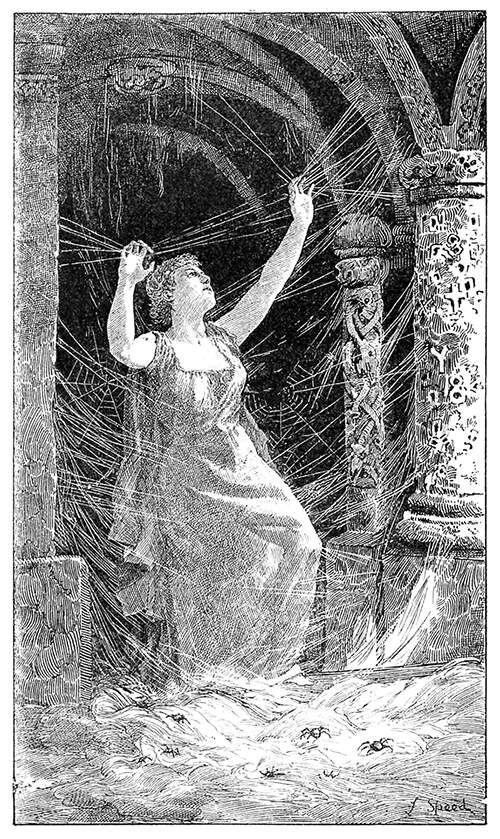
\includegraphics[width=2.5in]{images/cover}
\nbvspace[3]
\normalsize

\large
SESQUIPEDALIA VERBA PUBLISHING LTD
\nbvspace[1]
\end{center}

\setcounter{tocdepth}{2}
\cleardoublepage
\tableofcontents
\listoffigures
\addtocontents{toc}{~\hfill\textbf{Page}\par}

\mainmatter





\chapter{Introduction}
\label{intro}

\paragraph{} 

\chapter{Hello World}
\label{hello_world}
\paragraph{} We'll begin our series of projects with an exploration of `Hello World' but from a Flask perspective. Because we really can create a simple Flask app with nine lines of code, including white space, it's worth annotating every line here and going through each in turn. This will give us a firm and well understood foundation on which to build our subsequent projects.

\begin{lstlisting}
from flask import Flask 
app = Flask(__name__)

@app.route("/")
def hello():
    return "Hello World!"

if __name__ == "__main__":
    app.run(host='0.0.0.0')

\end{lstlisting}

\begin{description}
\item[Line 1] \emph{from flask import Flask}\\ 
Import the Flask class from the flask library. The library contains pre-written code and utilities that are useful when writing a web-app. In this case an instance of the Flask class will be our WSGI application.
\item[Line 2] \emph{app = Flask(\_\_name\_\_)}\\
Create an instance of the Flask class. The argument `\_\_name\_\_' is the name of the flask applications module. This is used to help flask to find resources relative to the Python module such as static web resources like image files, templates, or CSS. We also create a variable, `app', that references the newly instantiated Flask class so that we can use it later.
\item[Line 4] \emph{@app.route("/")}\\
Lines that start with @ in Python are decorators. In this case we use the route() decorator to tell Flask which URL should trigger the function that route() decorates, e.g. when a browser hits the root of the url, `/' then the hello() function is run. We use route() decorators in flask to build up our HTTP API that a browser can retrieve.
\item[Line 5] \emph{def hello():}\\
This defines a function called `hello()'. hello() is executed whenever someone requests the root url. This is because the function, hello(), and the decorator, @app.route(``/''), work together. Essentially when a request arraives to a matching decorator, e.g. to the root route, then the associated Python function is executed.
\item[Line 6] \emph{return "Hello World!"}\\
All our hello() does is to return the string ``Hello World!''. It is this string that is displayed in the browser. We could instead return some HTML for a richer experience but plain text is sufficient for now.
\item[Line 8] \emph{if \_\_name\_\_ == "\_\_main\_\_":}\\
This is used to control how the Python module and the flask app server is run. We only want to use app.run() if this script is executed from the Python interpreter, e.g. by calling \$python hello.py. If we were to use an app server instead then the app.run() would be performed differently.
\item[Line 9] \emph{app.run(host='0.0.0.0')
}\\
Calls the run() function of the Flask app class instance to start our development server running using this app as the web app. This line also tells the app to run on a network interface that is accessible from an external address, e.g. from the Windows machine that is running your SSH connection, otherwise our app would only be accessible within the dev server and we don't have a graphical browser installed there.
\end{description}

\paragraph{} Let's expand on hello world to make some of the concepts a little more firm. We'll make the string returned from the root route a little more generic, then we'll add two additional routes, one for hello, and one for goodbye, each of which will return a different, appropriate message when called.

\begin{lstlisting}
from flask import Flask 
app = Flask(__name__)

@app.route("/")
def greet():
    return "Greetings traveller"

@app.route("/hello")
def hello():
    return "Hello World!"

@app.route("/goodbye")
def goodbye():
    return "Goodbye cruel existence."

if __name__ == "__main__":
    app.run(host='0.0.0.0')

\end{lstlisting}

\paragraph{} What we've really done here is to build a simple HTTP API that supports creating dynamic individual responses to HTTP GET requests messages to three different routes, to `/', to `/hello', and to `/goodbye'. You could build an entire site in this way, just adding in the route decorators, to correspond to each web page that you want your site to support, and then creating a corresponding function for dynamically generating the actual page to return. Note that whilst the content of our dynamic pages is perhap less than dynamic, just strings like `Hello World!' and `Goodby cruel existence', the web pages themselves, returned to the calling client, which is most likely a web browser, are dynamically built by Flask when constructing the response object that is transmitted to close the current request-response cycle.

% DYNAMIC EXAMPLE - return a randomly selected greeting from a list of international greetings


% PERSONALISED EXAMPLE - return a personalised greeting (where the name is supplied in the URL

\chapter{Build a Quiz Site}
\label{quiz}
\paragraph{} In this chapter we'll explore a few different ways to build a quiz site using various features of Flask to iteratively elaborate our site.


\section{A Super Simple Quiz}
\paragraph{} We'll start with a super simple example. On each page you'll be asked a question, and you'll be presented with a selection of possible answers. Each answer is a link to another page. If you click the link which is the correct answer then you'll move to the next question and if you click an incorrect answer link then you'll move to a page telling you that your answer was incorrect and offering an opportunity for another go.

\paragraph{} This demonstrates how we can decompose the problem ``building a quiz'' into a simple hypertext site, needing neither javascript in the client nor additional python on the server, to provide a simple quiz game experience. We have, however, included a little bit of inline HTML for each page in order to get some visual interest and to enable us to create hyperlinks.

\paragraph{} Obviously there are many ways to create a web-based quiz site, and this is just one super simple approach that shows off some aspects of Flask. So let's take a look.

\begin{lstlisting}
from flask import Flask
app = Flask(__name__)

@app.route("/")
def hello():
    return """
    <h1>A Super Simple Quiz Example</h1>

    <p>Hi folks.</p>
    <p>Welcome to this super simple quiz site example. It's meant to be a really straightforward proof of concept that demonstrates the simplest kind of online quiz using just some basic Python & Pure Flask (i.e. no static files or templates. Minimal HTML, CSS, & JS).</p>

    <b>Do you want to play a game?</b>

    <a href="/q1/">Damn right I want to play a game!</a>
    """

@app.route("/q1/")
def q1():
    return """
    <h1>Question One</h1>
    <p>Which is the best university in Edinburgh?</p>

    <ul>
        <li><a href="/q2/">Edinburgh Napier</a></li>
        <li><a href="/q1w/">University of Edinburgh</a></li>
        <li><a href="/q1w/">Herriot Watt</a></li>
        <li><a href="/q1w/">Queen Margaret</a></li>
    <ul> 
    """

@app.route("/q1w/")
def q1w():
    return """
    <h1>Das ist der wrong answer!</h1>

    <a href="/q1/">Do you want to try again?</a>
    """

@app.route("/q2/")
def q2():
    return """
    <h1>Question Two</h1>
    <p>Which is the best university in Scotland?</p>

    <ul>
        <li><a href="/q3/">Edinburgh Napier</a></li>
        <li><a href="/q2w/">University of Edinburgh</a></li>
        <li><a href="/q2w/">Herriot Watt</a></li>
        <li><a href="/q2w/">Queen Margaret</a></li>
    <ul> 
    """

@app.route("/q2w/")
def q2w():
    return """
    <h1>That answer was a little lacking in correctness.</h1>

    <a href="/q2/">Do you want to try again?</a>
    """


@app.route("/q3/")
def q3():
    return """
    <h1>Question Three</h1>
    <p>Which is the best university in the UK?</p>

    <ul>
        <li><a href="/success/">Edinburgh Napier</a></li>
        <li><a href="/q3w/">University of Edinburgh</a></li>
        <li><a href="/q3w/">Herriot Watt</a></li>
        <li><a href="/q3w/">Queen Margaret</a></li>
    <ul>
    """

@app.route("/q3w/")
def q3w():
    return """
    <h1>Afraid not!</h1>
    <p>Perhaps consider whether there was a pattern forming amongst the answers to previous questions?</p>

    <a href="/q3/">Do you want to try again?</a>
    """

@app.route("/success/")
def success():
    return """
    <h1>You answered all the questions correctly</h1>
    <h2>Well done you</h2>

    <a href="/">Let's return to the home page</a>

    """

if __name__ == "__main__":
    app.run(host="0.0.0.0")
\end{lstlisting}


\paragraph{} This example demonstrates the following:

\begin{itemize}
\item How to create a number of routes. Remember that each route corresponds to a different web address on your site. For simple examples, each web address also corresponds to a different web page (and to a different Python function). You should be noticing how the route, function, and page are related and work together.
\item A simple way of breaking an idea, a quiz site, into a number of pages that are inter-connected using hyperlinks.
\end{itemize}


\section{A Simple Quiz Using HTML Files}
\paragraph{} This version of the quiz is almost identical to the previous one, however, to make things easier, we've moved all of the HTML content for the pages out of the Python script, and into their own individual HTML files, one for each page. These HTML files are stored in their own sub-folder named `templates'. The templates folder is the default location\footnote{although this can be overridden} in which Flask looks for HTML templates. Flask will serve up any matching HTML file in the template folder when the render\_template() function is called. Note that a template is an HTML file that possibly contains additional JINJA2 code directives to dynamically alter the HTML content. However, we don't have any Jinja2 directives in our HTML files at this point, so our templates are the most straightforward that we can create, raw and valid HTML, which will be returned unaltered to our calling client.

\paragraph{} The project is organised as follows. We have a project folder containing our quiz.py script and a sub-folder called ``templates''. In the templates folder are eight HTML files that represent the pages of our quiz site.

The `quiz.py' file listing is as follows:

\begin{lstlisting}
from flask import Flask, render_template
app = Flask(__name__)

@app.route("/")
def hello():
    return render_template('index.html')

@app.route("/q1/")
def q1():
    return render_template('q1.html')

@app.route("/q1w/")
def q1w():
    return render_template('q1w.html')

@app.route("/q2/")
def q2():
    return render_template('q2.html')

@app.route("/q2w/")
def q2w():
    return render_template('q2w.html')

@app.route("/q3/")
def q3():
    return render_template('q3.html')

@app.route("/q3w/")
def q3w():
    return render_template('q3w.html')

@app.route("/success/")
def success():
    return render_template('success.html')
    
if __name__ == "__main__":
    app.run(host="0.0.0.0")
\end{lstlisting}

\paragraph{} This is a simple Flask app, very similar to the previous Quiz example, but we've extracted the HTML from within the Python file. The HTML is now stored in their own separate HTML files, one for each page. To send a specific HTML file back to the caller we use the render\_template() function passing in the name of the template to send. Note that each of our routes corresponds to a different page of the site and that each route returns a different template, hence, a different page.

\paragraph{} The `/' route is the index page, then we've named our other routes and associated functions to help keep track of their functionality, e.g. `/q1/' is question 1, and `/q1w/' is the page for incorrect answers to question 1. The same pattern is used for questions 2 and 3. Finally their is a success page that is reachable from the `/success/' route.

\paragraph{} Let's take a look at the contents of the `index.html' page:

\begin{lstlisting}
<!DOCTYPE html>
<html>
<head></head>
<body>
    <h1>A Super Simple Quiz Example</h1>

    <p>Hi folks.</p>
    <p>This time, instead of returning our HTML code as strings from our Python routes/functions, we've extracted the HTML code, topped and tailed it into complete HTML files, and placed them in the templates folder.</p>

    <b>Do you want to play a game?</b>

    <a href="/q1/">Damn right I want to play a game!</a>
</body>
</html>
\end{lstlisting}

\paragraph{} Note how the index page links directly to the first question page `q1.html', which is shown here:

\begin{lstlisting}
<!DOCTYPE html>
<html>
<head></head>
<body>
    <h1>Question One</h1>
    <p>Which is the best university in Edinburgh?</p>

    <ul>
        <li><a href="/q2/">Edinburgh Napier</a></li>
        <li><a href="/q1w/">University of Edinburgh</a></li>
        <li><a href="/q1w/">Herriot Watt</a></li>
        <li><a href="/q1w/">Queen Margaret</a></li>
    <ul>
</body>
</html>
\end{lstlisting}

\paragraph{} Note how each anser leads to a different page, the question 2 page for the correct answer and the question 1 wrong page for all other answers. The `q1w.html' page is shown here:


\begin{lstlisting}
<!DOCTYPE html>
<html>
<head></head>
<body>
    <h1>Das ist der wrong answer!</h1>

    <a href="/q1/">Do you want to try again?</a>
</body>
</html>
\end{lstlisting}

\paragraph{} Note how this page displays a message informing the player that they are wrong, and offers a link back to try answering the question again.

\paragraph{} The remaining HTML pages are similarly structured so it is worth investigating them in the Git repository and making sure you have a good understanding of how each works, both in terms of internal structure of a single page, but also how each page, through hyperlinks, connect to other specific pages that make up the site. In this way the hyperlinks between pages make up an aspect of the site's functionality.



\section{A Simple Quiz Using Static Files}
\paragraph{} This example expands upon the previous one and still includes both the HTML files in the templates folder and the core quiz.py script. However we've also added a static sub-folder as a sibling to the templates folder. Into this, for organisation purposes we have a sub-folder called `css', to store our CSS files which we'll beed to add some style to our HTML. CSS files are static because, at least in our current context, they won't change as a result of our Flask app running, and will generally remain the same whilst the site is being used. Javascript files are also considered static, as are image files, font files, and anything else that isn't being generated or altered by our Python code\footnote{Note that you could have CSS, JS, images, etc generated on the fly directly from code but under normal circumstances theses are generally considered to be fairly static parts of a web-site.}.

\paragraph{} Our quiz.py hasn't altered since the last example, our only changes this time around are within the HTML files, to indicate where the new CSS style files are located. So let's first look at the CSS file and then we'll look at a representative example of an HTML template file using that style file.

\paragraph{} In the static folder you will see a css folder. Within that folder you will find style.css which has the following contents:

\begin{lstlisting}
body{
    max-width:650px;
    margin:40px auto;
    padding:0 10px;
    font:18px/1.5 -apple-system,BlinkMacSystemFont,"avenir next",avenir,"Segoe UI","lucida grande","helvetica neue",helvetica,"Fira Sans",roboto,noto,"Droid Sans",cantarell,oxygen,ubuntu,"franklin gothic medium","century gothic","Liberation Sans",sans-serif;
    color:#444
    }
h1,h2,h3{line-height:1.2}

\end{lstlisting}

\paragraph{} This is fairly standard CSS to make our page look a little better than raw HTML. Obviously you can include whicheve CSS directives you want but this is meant to be a simple demonstration that improves on the default HTML style. We've set a max-width for the body, added a margin and some padding, specified some fonts, and a background colour. We've also set the line heigth for the level 1, 2, and 3 headings.

\paragraph{} How do we get our HTML templates to use this style? Let's look at a representative example, the `index.html' file:

\begin{lstlisting}[]
<!DOCTYPE html>
<html>
<head>
    <link href="{{ url_for('static', filename='css/style.css') }}" rel="stylesheet" />
</head>
<body>
    <h1>A Super Simple Quiz Example</h1>

    <p>Hi folks.</p>
    <p>This time, instead of returning our HTML code as strings from our Python routes/functions, we've extracted the HTML code, topped and tailed it into complete HTML files, and placed them in the templates folder.</p>

    <b>Do you want to play a game?</b>

    <a href="/q1/">Damn right I want to play a game!</a>


</body>
</html>
\end{lstlisting}

\paragraph{} We've added a link element into the head element of the page. Notice that this isn't just a regular HTML element though. This also includes a Jinja2 directive \emph{\{\{ url\_for('static', filename='css/style.css') \}\}}. Jinja2 uses double opening and closing curly braces ``\{\{'' and ``\}\}'' to delimit the start and end of Jinja2 code, which is interspersed within the HTML. In this case Jinja2 is using the url\_for() function to construct a hyperlink to place into the HTML at this point. It is also specifying that a specific file be referenced by this link, style.css, and that the file is located in the static folder. ALso notice that because style.css is in it's own `css' sub-folder within the static folder, we've just added the extra path information in the \emph{filename=} clause.

\paragraph{} If you example the other HTML files in the templates folder you'll see that a similar Jinja2 directive is used. This means that every HTML file is linking to the same CSS style file. The same mechanism can be used to reference any files that you place in your static folders, so if you want to include an image, e.g. a png or jpg file, or a javascript file, then you can use the url\_for() function in a similar way to place the correct path within the correct HTML hyperlink.


\section{A slighly more complex Quiz}
\paragraph{} This example is largely similar to the previous examples but makes some significant changes. Firstly, the static folders and CSS remain the same. However one might ask, why do we need an HTML file for each question if each page is actually similar. Couldn't we just create a template to represent, e.g. a generic question page, and then dynamically fill out the template with details when the page is called? Yes we can. It turns out that this is at the heart of the idea of dynamically and efficiently creating web pages using Flask.

\paragraph{} Firstly, example the templates folder. Notice that there are just four templates in our folder, half as many as previously. We still have an index.html and a success.html page, but now we have a generic quiz.html template used for each question page in the quiz and a generic `wrong answer' page, used when a player makes a poor choice of answer. Let's briefly look at the quiz and wrong answer pages in turn:


\begin{lstlisting}
<!DOCTYPE html>
<html>
<head>
    <link href="{{ url_for('static', filename='css/style.css') }}" rel="stylesheet" />
</head>
<body>
    <h1>Question {{ number }}</h1>
    <p> {{ text }} </p>

    <ul>
        
        <li><a href="/quiz/?answer={{loop.index}}">{{ answer }}</a></li> 
        
    <ul>
</body>
</html>

\end{lstlisting}

\paragraph{} Notice that in this template we now have three additional Jinja2 directives in addition to the one for the stylesheet link. To find the Jinja2 directives just look for the double curly braces. The first directive is in the $<$h1$>$> element and gives a placeholder for a question number to be inserted. The next directive is in the paragraph element and is a placeholder for question text. The final directive is a little more complex and uses a for loop to iterative over a list of answers, adding each as a list item in an HTML unordered list. This one is also more complex because it is made up of a few additional Jinja2 directives to specify a number in each $<$a$>$ tag and to create a placeholder for the answer text.

\paragraph{} Now let's take a look at the wrong answer template in the wrong.html file:

\begin{lstlisting}
<!DOCTYPE html>
<html>
<head>
    <link href="{{ url_for('static', filename='css/style.css') }}" rel="stylesheet" />
</head>
<body>
    <p> {{ text }} </p> 

    <a href="/">Let's return to the home page</a>
</body>
</html>

\end{lstlisting}

\paragraph{} This just has a single additional Jinja2 directive to allow some text to be placed within a paragraph element.

\paragraph{} In both templates, the data to use with the Jinja2 directive, e.g. the text to place in the paragraph, is supplied by the calling function in our Python Flask script.

\paragraph{} Now let's look at the quiz.py script. There've been some fairly major alterations here to enable us to make better use or our templates, and also, more importantly, we're now checking whether the answer is correct on the server and generating the response depending upon whether the player was right or wrong.

\begin{lstlisting}
from flask import Flask, render_template, request, session
app = Flask(__name__)
app.secret_key = 'SUPERSEKRETKEY'


@app.route("/")
def hello():
    session['question'] = 1
    return render_template('index.html')


@app.route("/quiz/")
def quiz():
    q = None
    qa = {
        "1":{
            "text":"Which is the best university in Edinburgh?",
            "answer":1,
            "answers":["Edinburgh Napier", "University of Edinburgh", "Heriott Watt", "Queen Mary" ]
        },
        "2":{
            "text":"Which is the best university in Scotland?",
            "answer":1,
            "answers":["Edinburgh Napier", "University of Edinburgh", "Heriott Watt", "Queen Mary" ]
        },
        "3":{
            "text":"Which is the best university in the UK?",
            "answer":1,
            "answers":["Edinburgh Napier", "University of Edinburgh", "Heriott Watt", "Queen Mary" ]
        },
        "4":{
            "text":"Which is the best university in the World?",
            "answer":1,
            "answers":["Edinburgh Napier", "University of Edinburgh", "Heriott Watt", "Queen Mary" ]
        }
    }
    try:
        if (session['question']):
            q = int(session['question'])
    except KeyError:
        q = 1

    answer = request.args.get('answer', None)
    if answer is not None:
        correct = qa.get(str(q)).get('answer')
        if str(answer) == str(correct):
            q = q+1
            session['question'] = q
            if q > len(qa):
                return render_template('success.html')
            else:
                return render_template('quiz.html', text=qa[str(q)]["text"], answers=qa[str(q)]["answers"], number=q)
        else:
            return render_template('wrong.html', text="Das ist der wrong answer!!!")
    else:
        return render_template('quiz.html', text=qa[str(q)]["text"], answers=qa[str(q)]["answers"], number=q)


@app.route("/success/")
def success():
    return render_template('success.html')
    

if __name__ == "__main__":
    app.run(host="0.0.0.0")
\end{lstlisting}

\paragraph{} Note that the root and success routes have not been altered greatly. The root route sets the current question in the session object to `1' but there are no further changes. All of the substantive changes in this version are in the new `/quiz/' route which is the heart of our quiz game.

\paragraph{} Lines 15 to 36 are a dictionary containing the questions and answers for our quiz. The `text' key is the text of the question, `answer' is the number of the answer in our answer list, and `answers' is a list of possible answers. Lines 37 to 41 check for a valid session and retrieve the current question if it exists or else set the current question to 1 if it doesnt'. The quiz route uses a URL argument parameter to communicate the players answer number back to the server, so we retrieve this in line 43. At this point we branch depending whether there is an answer or not. If not then we display page for the current question (line 56). Otherwise we check the answer, if it is wrong we render the template for the wrong answer and return it (line 54). If the answer is correct and there are more questions then we render the template for the next question (line 52) and if we've run out of question then we render the template for the successful culmination of the quiz (line 50). Note in the render\_template() calls how we supply various additional bits of data? These are the data that the Jinja2 directives use to complete the template into a fully-formed HTML page. This extra data in the render\_template() function is our conduit from Python code, data, and variables into our HTML templates.



%\begin{lstlisting}
%\end{lstlisting}


\chapter{Serendipity}
\label{serendipity}
\paragraph{} Serendipity is the occurence and development of events by chance in a happy or beneficial way. Sometimes, when creating things, or uncertain, we can attempt to harness serendipity to help us to side-step indecision. This inspires the example project that we'll build in this chapter, a simple site to provide us with cues to help us to make decisions when we're unsure. We'll use this as a scenario for developing an API including a small example user interface and an HTTP/JSON interface.

\paragraph{} Our two main sources of serendipity in this project will be the `Magic 8 Ball' and Brian Eno's `Oblique Strategies'. The magic 8 ball is a toy to which you direct a question, and the result is some random response from a list of supportive, neutral, or dismissive responses.
The oblique strategies are fairly similar, but are intended to help you to find creative ways around an impasse, perhaps in a design or other creative endeavour. Whilst the magic 8 ball started out as a toy, the oblique strategies came from musicians who were looking for interesting and creative ways to solve problems and make interesting sounds.

\paragraph{} From the Flask perspective, the aim of this chapter is to explore some elements involved in building a simple HTTP based API. We'll create a few routes and associated functions, that will demonstrate:

\begin{enumerate}
\item How to build a simple JSON API
\item How to build a simple form-based UI
\item How to integrate flask routes and non-flask Python functions
\end{enumerate}


\section{Code Listing}
\paragraph{} The following code listing is nearly complete. The only parts missing are the contents of the full lists of magic 8 ball responses and oblique strategies because they take up a lot of space. These elided parts are indicated in lines 85 and 94 where the missing elements are replaced by an ellipsis. The full source code listsing is available from the Git repo.

\begin{lstlisting}
from flask import Flask, request, jsonify
import random, json

app = Flask(__name__)

@app.route("/")
def index():
    return """
    <h1>A Serendipity API & Inteface</h1>
    """, 200    


@app.route("/query/", methods=['GET', 'POST'])
def query():

    if request.method == 'POST':
        page='''
            <!DOCTYPE html>
            <html><body>
            <h1>Your question was:
        '''
        page+=request.form['question']
        page+='''
            </h1>
            <h1>Your answer is:
        '''
        page+= amalgamate()
        page+='''
            </h1>
            <body></html>

        '''        
        return page
        
    else:
        page='''
            <!DOCTYPE html>
            <html><body>
                <form action="" method="post" name="form">
                    <label for="question">Question:</label>
                    <input type="text" name="question" id="question"/>
                    <input type="submit" name="submit" id="submit"/>
                </form>
            <body></html>
        '''
        return page


@app.route("/magic8ball/", methods=['GET','POST'])
def magic8ball_page():

    if request.method == 'POST':

        question = request.get_json().get("question")
        
        data = {
            "question": question,
            "answer": magic8ball()
        }
        return jsonify(data), 200

    else:
        data = {
            "answer": magic8ball()
        }

        return jsonify(data), 200


@app.route("/oblique/")
def oblique_strategies_page():

    data = {
        "strategy": oblique_strategies()
    }

    return jsonify(data), 200



def magic8ball():
    responses = [
        "It is certain.", 
        "It is decidedly so.",
        ...
        "Very doubtful."
    ]
    return random.choice(responses)

def oblique_strategies():
    strategies = [
        "Abandon normal instruments",
        "Accept advice",
        ... 
        "[blank white card]"        
    ]
    return random.choice(strategies)

def amalgamate():
    functions = [magic8ball, oblique_strategies]
    return random.choice(functions)()

if __name__ == "__main__":
    app.run(host="0.0.0.0")
\end{lstlisting}

\section{Structural Overview}
\paragraph{} The serendipity webapp defines seven functions. Of these, four of the functions are also Flask routes. The remaining functions are pure Python functions that are called and utilised when our webapp runs. For example, the magic8ball() function is called by the magic8ball\_page() function, which in turn is invoked when the \emph{/magic8ball/} route is called by a client, such as a browser, making a request to that specific route. Take a moment to familiarise yourself with the overall structure of the code, the different functions and how the functions that are also web routes are delineated from those that are not.

\subsection{/ Route}
\paragraph{} This is a simple root route that contains a single $<$h1$>$ element naming the webapp. It doesn nothing more. The only point of interest here is that we have used a multi-line Python string, and that we are explicitly returning a 200 status code alongside the response.

\subsection{/query/ Route}
\paragraph{} The questy route responds to both HTTP GET and HTTP POST requests. When a GET request arrives a web page is displayed. We've defined the HTML inline in a multiline Python string, but a template would work even better. The displayed page contains a simple form with a label, a text entry (for the question), and a button to initiate the POST. This form is POST'ed to the same route, the /query/ route and so, because form submissions are POSTs by default, the other part of the query() function is executed, the part that checks for and handles POST requests. The if clause that handles POST requests builds an HTML page inline, again using Python's multiline strings. However this time we build the page bit by bit, using the `+=' operator to append new information to the end of the string that represents our HTML page. In this way we can insert data wherever it is required in the HTML. For example, in line 22 we append the question from the user submitted form, and in line 27 we make a call to the amalgamate() function. When done we return the entire page as our HTTP response to the client.

\subsection{/magic8ball/ Route}
\paragraph{} This route responds to both HTTP GET and HTTP POST requests. So it requires an if clause to immediately determine whether the incoming request is a GET or a POST. If the request is a GET then it creates a dictionary containing a single key:value pair. The key is ``answer'' and the value is one randomly selected magic 8 ball response returned by a call to the magic8ball() function. This dictionary is then turned into a HTTP response containing a JSON string as it's payload using the Flask jsonify function. POST is similar but has some additional functionaliy. This POST request includes a POST'ed JSON request body that contains a single key:value pair \{ ``question'':``\emph{question content}'' \}. The value is extracted from this pair, using the request.get\_json() function, and is used to add an extra key"value pair to the data dictionary alongside the magic8ball response. To summarise, we're extracting the question from the incoming POST request, adding the question to our data dictionary, getting a random magic 8 ball answer and adding that to our data dictionary, then turning the entire dictionary into JSON and returning it to the client in our response.

\subsection{/oblique/ Route}
\paragraph{} This route responds to HTTP GET requests only. It creates a dictionary containing a single key:value pair. The key is ``strategy'' and the value is one randomly selected oblique strategy returned by a call to the oblique\_strategies() function. This dictionary is then turned into a HTTP response containing a JSON string as it's payload using the Flask jsonify function.


%\section{Line-By-Line Annotation}


%\begin{lstlisting}
%\end{lstlisting}

%\begin{description}
%\item[Line 1] \emph{}\\ 
%\end{description}





\backmatter

\bibliographystyle{plain}

\bibliography{bib/flask}

\end{document}

